\chapter{Poroelastic natural coatings}

\chapquote{Nature is the source of all true knowledge. She has her own logic, her own laws, she has no effect without cause nor invention without necessity}{}{Leonardo Da Vinci}

\section{Biomimetics of poroelastic coatings}

Usually when someone is asked to imagine some "rapid" object as an airplane, a boat or a car, the common sense lead us to think about it as the smoothest as possible and most of the time shiny.
But if we look around us the nature seems not to agree with the previous statement.
In fact most of the surfaces in nature are not smooth at all, they present almost always some kind more or less regular arrangement of discontinuities at various length scales.
Since Nature have had a very large time-span to optimize this kind of surfaces we can be very certain that they are the best possible option.
One should pinpoint that the non smoothness of these surfaces can be connected to some other biological functions rather than pure fluid dynamic performance, and of course it can be the case.


With that in mind we want to show to the reader some of the most notably examples of "natural" aerodynamically surfaces.

Probably the most notable example is the shark skin, in figure \ref{fig:shark} a segment of the skin is depicted as if appears to be under the microscope.

\begin{figure}[h]
	\centering
	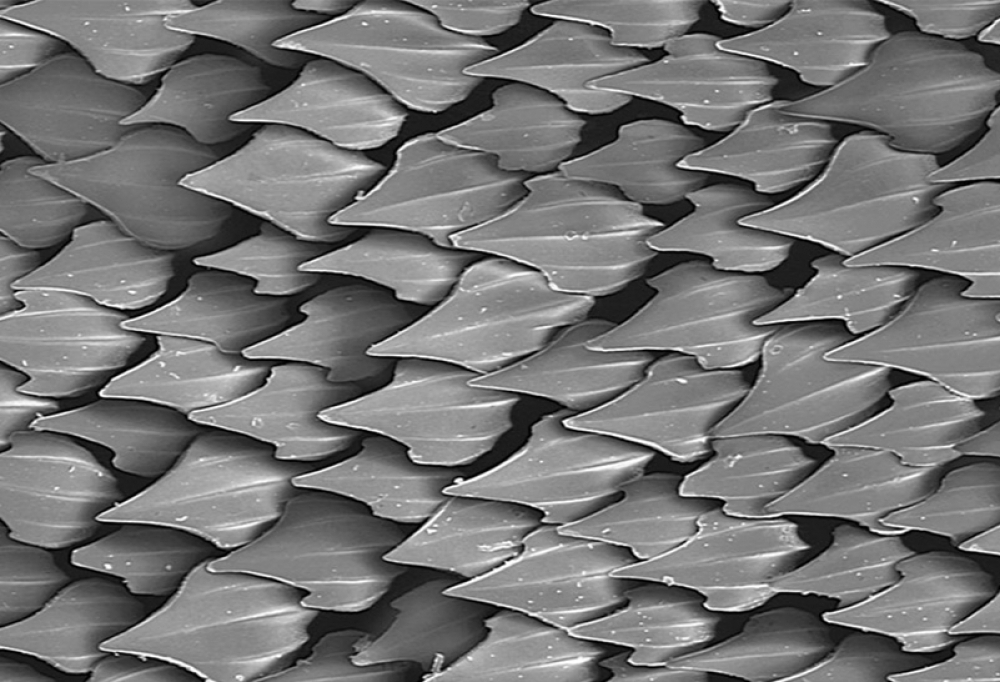
\includegraphics[width=0.6\linewidth]{chapter_1/shark}
	\caption{Microscope enlarged picture of the shark skin.}
	\label{fig:shark}
\end{figure}

The enlargement show that the surface is made up by a series of overlapped denticles, and experiment shows that they can move and interact with the flow.

The shark technology has somehow been applied by Speedo$^{\circledR}$ in their famous swimming suits, that had break multiples world records.
But it seems that this controversial swimmers performance came more on the compressed and streamlined body shape than from the surface texture itself.
In fact during the years this texture material has been publicized to be like synthetic shark skin but \cite{Oeffner785} has shown that the texture is somehow different from the shark dermal structure.
They have also performed some swimming experiment with a flat plate with different surfaces and they have found no significant speed enhancement with the swimsuit surfaces; but the measurements with the shark skin on the contrary give an appreciable improvement in the performance.


Poroelastic surfaces find also applications in aeroacoustics, in fact the owl is well known for its particularly silent flight, in the high frequency spectrum.
This characteristic is crucial for the owl in order to be able to capture his preys.
Obviously it has inspired the scientific community to study the feathers configuration and their shape.

\begin{figure}[h]
	\centering
	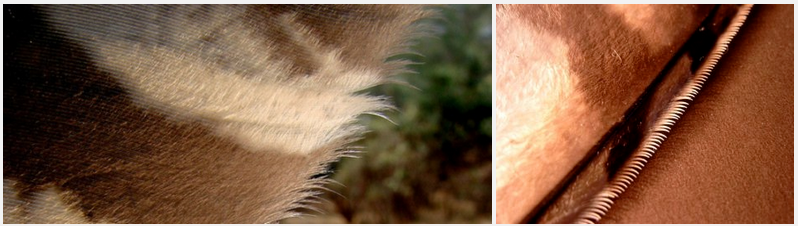
\includegraphics[width=0.8\linewidth]{chapter_1/howl}
	\caption{Feathers in owl's wing: trailing edge (left), leading edge (right). The difference in shape, and mechanical properties as rigidity, between the leading and trailing edge is a consequence of the different flow regimes in the wing.}
	\label{fig:owl}
\end{figure}
 
Multiple authors show promising result in characterizing the acoustic properties of the owl skin and their physical mechanism.
In particular \cite{lilley1998} present three main characteristic of the owl that can suppress its airborne noise: the feathers leading edge shaped like a comb, the feathers trailing edge that form a fringe and the presence of multiple "filaments" in the bottom surface of the wing and on its legs.
in the same work he also present some experimental and empirical evidence on the aeroacoustics mechanism behind the three elements above.

Another examples of work in the field of owls acoustic is the one by \cite{jaworski2013aerodynamic} in which the authors study the acoustic scattering problem of a poroelastic half-plane hit by an incident plane wave.
This configuration has been used as an analogy with the owl wing, it try to explain how the properties of this surface can suppress the noise.
They conclude that the combined effects of elasticity and porosity can produce the weakest edge noise amplification.

Recent computational simulation made by \cite{rao2017owl} confirm that the leading edge shape of the feathers truly suppress noise and enhance the lift generation for angles of attack grater then $15^{\circ}$.


Bioinspired aerodynamic surfaces include another peculiar example in the butterflies wings.
In figure \ref{fig:butterfly} the surface of a "Peacock butterfly" is enlarged in order to show the multiple scales involved; the wing structure present firstly as overlapped scales similar to the shark, but looking closely we can observe that the singles scales have a complicated permeable structure.

\begin{figure}[h]
	\centering
	\begin{subfigure}[b]{0.3\textwidth}
		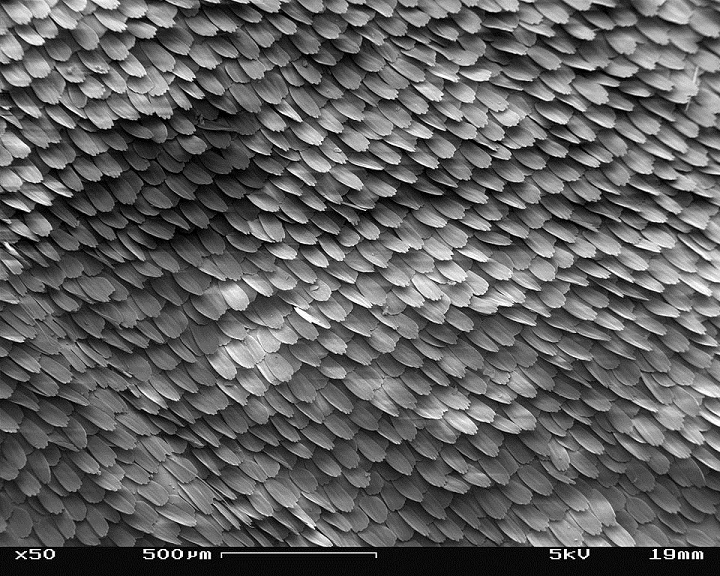
\includegraphics[width=\textwidth]{chapter_1/butterfly}
		\caption{Magnification 50x}
		\label{fig:b50}
	\end{subfigure}
	~ %add desired spacing between images, e. g. ~, \quad, \qquad, \hfill etc. 
	%(or a blank line to force the subfigure onto a new line)
	\begin{subfigure}[b]{0.3\textwidth}
		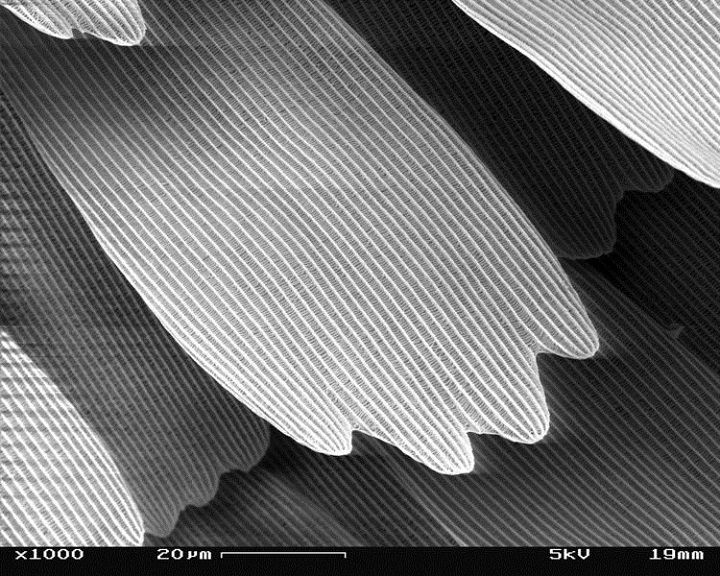
\includegraphics[width=\textwidth]{chapter_1/butterfly2}
		\caption{Magnification 1000x}
		\label{fig:b1000}
	\end{subfigure}
	\begin{subfigure}[b]{0.3\textwidth}
		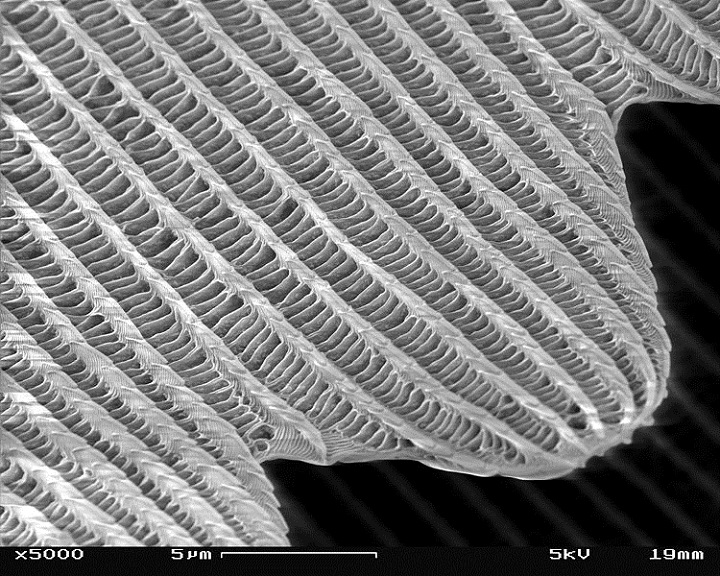
\includegraphics[width=\textwidth]{chapter_1/butterfly3}
		\caption{Magnification 5000x}
		\label{fig:b5000}
	\end{subfigure}
	\caption{Peacock butterfly wing surface using Scanning Electron Microscopy.  Images from wikimedia.org}
	\label{fig:butterfly}
\end{figure}

The work of \citet{slegers2017beneficial} the authors study the effect of such porous structure in the flight performance of butterflies.
Using cameras to measure the kinematics of their flight, they can compute their efficiency to "climb" (generate lift) and the stroke amplitude and frequency.
The authors conclude, after the proper statistical tests on the overall butterfly population, that the porous structure of their wing gives a boost in climbing efficiency about $30\%$; that results clearly stress out the importance of the poroelastic layer of the wings. 
Even though the flight aerodynamic is extremely complex \cite{srygley2002unconventional}, it seems clear that the peculiar structure of the wings surface is critical for their aerodynamic performances.


Superhydrophobic surfaces works as they were water repellent, in fact over such surfaces the water can slide over with much less resistance resulting in very small values of wettability.
This behavior is caused by the microscopic structure that forms the surface \ref{fig:lotus}, in fact the rugosities are arranged in a more or less regular way in order to be able to capture air pockets that rest inside this structures.
These air inclusion provoke an effective slip at the air-liquid interface that cause the drag reduction; but they also change the contact angle of droplets 
The work of \citet{bottaro2003effect} summarize the above aspect and their applications.

\begin{figure}[h]
	\centering
	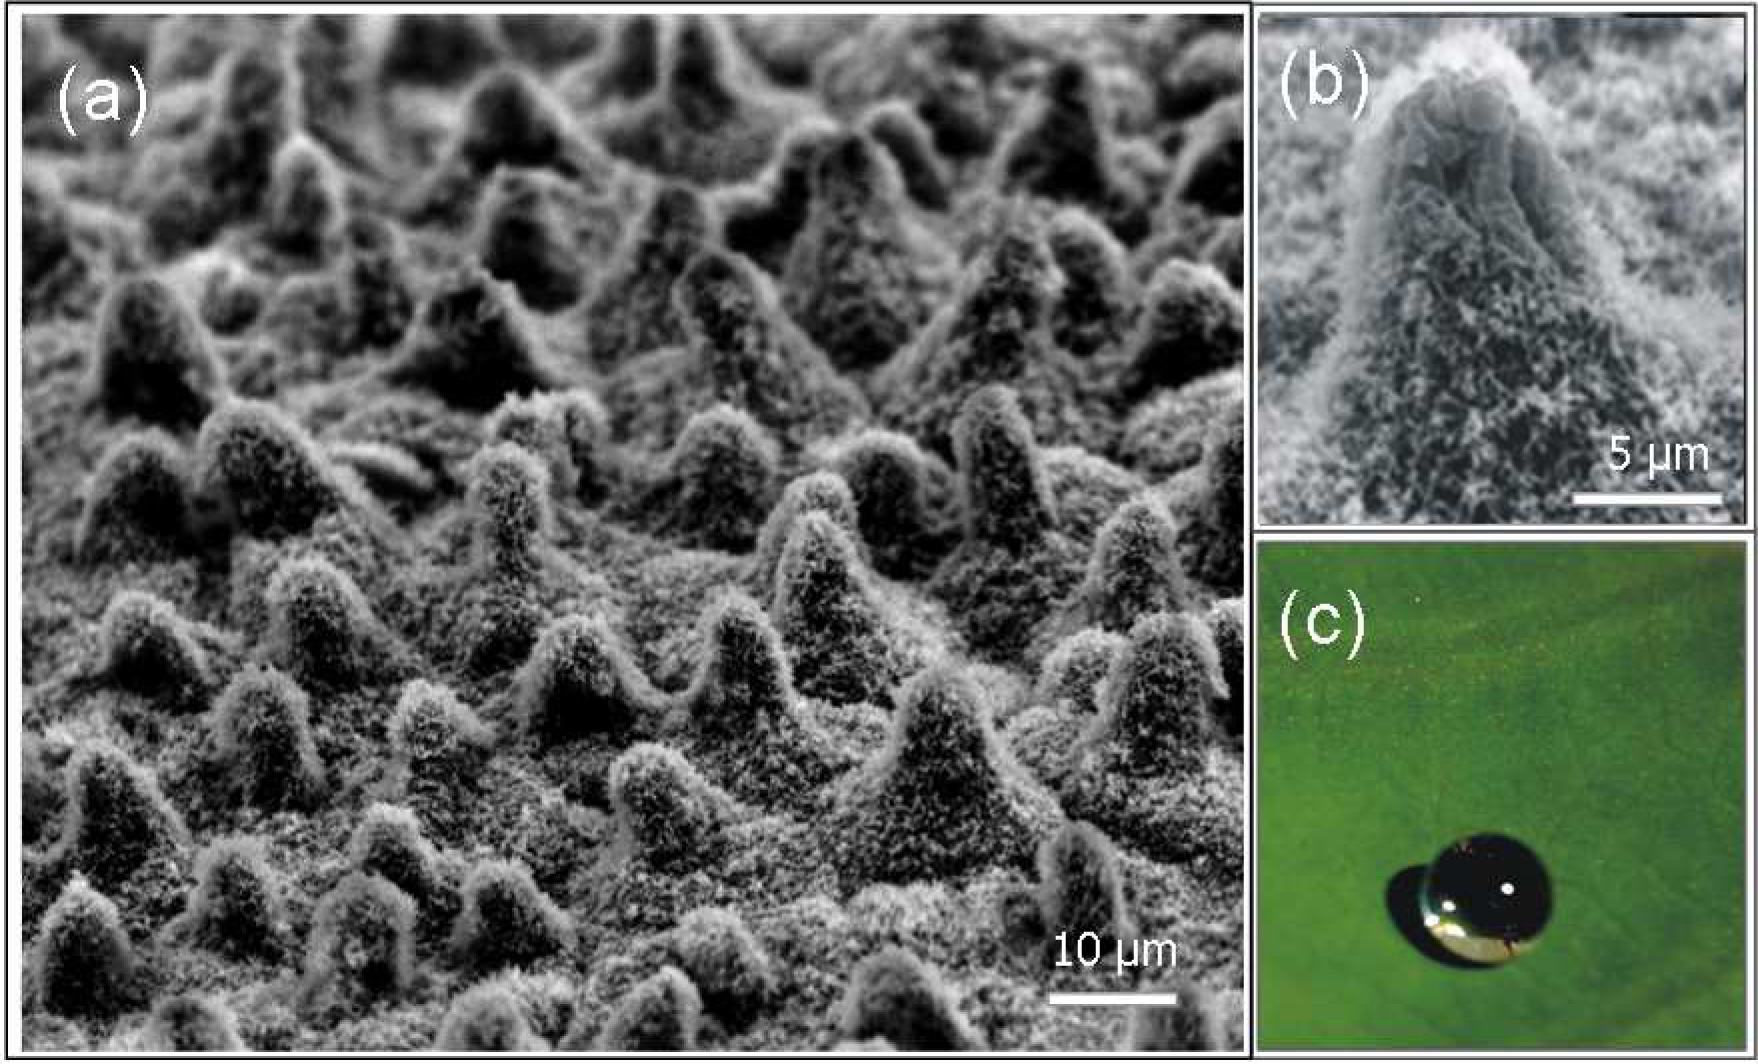
\includegraphics[width=0.6\linewidth]{chapter_1/lotus}
	\caption{(a) Scanning electron microscopy (SEM) image showing the structure of lotus leaf, (b) higher order of magnification on the single protuberance forming the surface and (c) a water drop that due to the contact angle attain an almost spherical shape. Images from \cite{stratakis2009laser}}
	\label{fig:lotus}
\end{figure}


The interest reader could find other examples and broaden the above key aspect also in \cite{bhushan2016biomimetics}, \cite{tropea2012nature}.

TALK ABOUT THE RESULTS IN \citet{segura2017permeable}

\subsection{Riblets and shark-skin surfaces}

We have seen that natural surface can be an inspiration to find strategies to solve many aerodynamics problems; in the following we will focus especially on the drag reduction.

Is known that the total drag contribution can be separated in different components, and the classical decomposition is between viscous drag (sometimes referred as skin friction) and pressure drag.

\begin{equation}
 \int_{A_{\sigma}}  [ \underbrace{\left( \frac{p}{\rho} \mathbf{I} \right) \cdot  \mathbf{n}_{\sigma} }_\text{pressure drag}  +  \underbrace{ \left( \nu \nabla \mathbf{v} \right) \cdot  \mathbf{n}_{\sigma}}_\text{viscous drag} ] \; dA,
 \label{eq:force}
\end{equation}

Where $A_{\sigma}$ is the solid interface of some body where a no slip condition is applied, and $ \mathbf{n}_{\sigma}$ is its outward normal.
In this section we will talk about the existing possible ways to reduce the viscous part of the drag since historically has attract more interest and/or make more progress.

In the following we will refer as the wall shear stress in the turbulent case as:
\begin{equation}
\tau = \left( \left( \mu + \mu_t \right)  \nabla \mathbf{\overline{v}} \right) \cdot  \mathbf{n}_{\sigma} = \left( \mu + \mu_t \right) \derp{\overline{u}}{y}
\end{equation}

where $\mu_t$ is the turbulent viscosity and $\overline{u}$ is the average velocity stramwise component; in the laminar case obviously the definition rest the same with some correction (there is no turbulent viscosity and no notion of average velocity).
Also $\mathbf{n}_{\sigma} = (0,1,0)$ is the conventional orientation in the literature.

Most of the industrial application involves turbulent flow; obviously there is a lot of research that aim to reduce the skin-friction in this regime.
Table 6.3.1 in the book of \citet{mclean2012understanding} make a wide list of technique already been proposed on the problem.

As the same author pinpoint the most effective, and probably the most practicable concept, are the riblets.
They are regularly arranged alternating ridges aligned in the streamwise flow direction as the figure \ref{fig:riblets1} show.

These surfaces are capable of align the turbulent flow in the mean flow direction smoothing the fluctuation of the cross-flow in the viscous sublayer.
Reducing this fluctuations close to the surface the turbulent momentum transfer will also be reduced and so the shear stress, causing the reduction in skin-friction.

\begin{figure}[h]
	\centering
	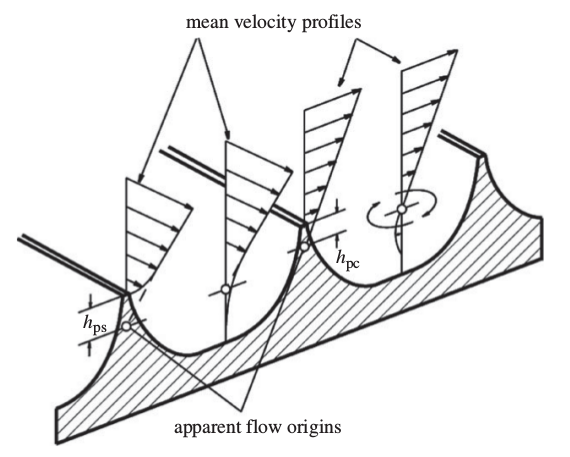
\includegraphics[width=0.7\linewidth]{chapter_1/riblets3}
	\caption{Schematics of the concept of \textit{protusion height}. The mean velocity profiles for the streamwise and crossflow velocities are presented. Where they are in the presence of a ridge is it possible to extrapolate the point of zero velocity from the velocity gradient outside the riblet, finding respectively the \textit{streamwise protusion height} $h_{ps}$ and the \textit{crossflow protusion height} $h_{pc}$. Image from \citet{bechert1997experiments}}
	\label{fig:riblets1}
\end{figure}


The viscous drag reduction correlates well with the spacing between the ridges expressed in wall units $ s^+ $, the typical shape is depicted in \ref{fig:riblets_perf} where the vertical axis show the drag reduction computed against the smooth surface case against the $ s^+ $.
This general shape of the curve, in which the skin friction decrease in certain range of spacing and then increase as the $ s^+ $ increase, is caused by a competition between the capacity of riblets to obstruct lateral fluid flow and an increase in the penetration of high speed vorticies inside this manufactured rugosities.

\begin{figure}[h]
	\centering
	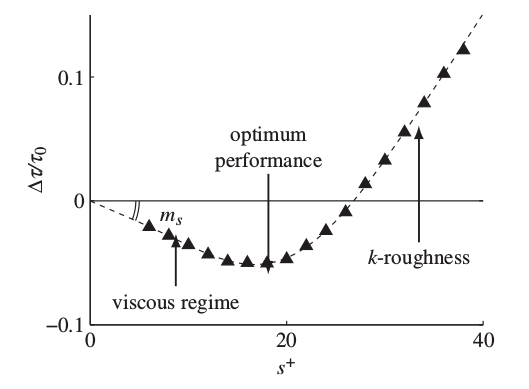
\includegraphics[width=0.5\linewidth]{chapter_1/riblets_performance}
	\caption{Performance ... \citet{jimenez2001turbulent} }
	\label{fig:riblets_perf}
\end{figure}

This last physical explanation of the riblets performances is presented in the schematics \ref{fig:riblets_schem}, where the grey areas show high skin-friction regions caused by the downwash motion generated by the near-wall vortices.
Is it clear that when the riblets are too big the vortices can penetrate inside its groove and actually increase the skin-friction due to larger area exposed to the local velocity.
On the contrary when the riblets are smaller, the high speed vortices "touch" only the tip of the ridges so only a small local area of the surface experience high-shear stresses.

\begin{figure}[h]
	\centering
	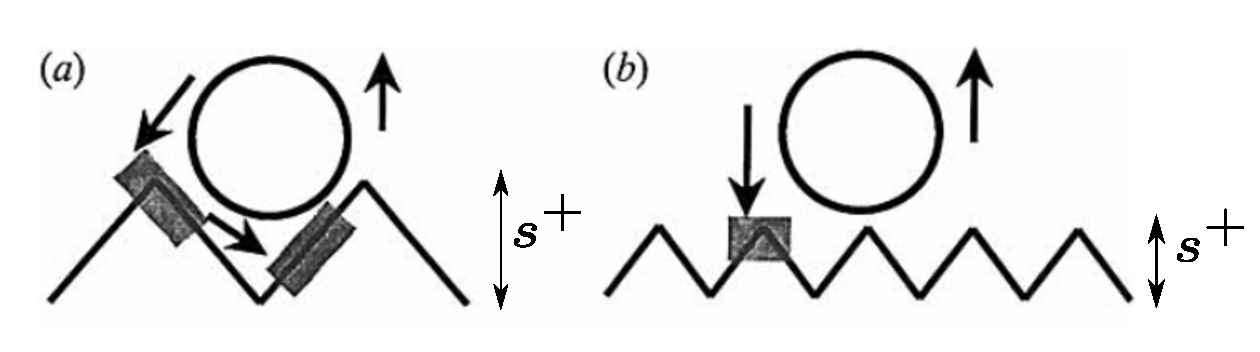
\includegraphics[width=0.7\linewidth]{chapter_1/riblets1}
	\caption{Two different size of riblets are represented interacting with a sublayer vortex. In grey is it represented the areas where the friction is important; clearly when the size of two is comparable (as the left picture) the surface experience a larger friction and the performance is lowered. Image from \citet{choi1993direct}}
	\label{fig:riblets_schem}
\end{figure}

The slope $m_s$ of the curve \ref{fig:riblets_perf} can be predicted by linear stability theory or by means of empirical correlations as in \citet{garcia2011hydrodynamic}.

Computing the performance of such surfaces can be expensive since the most reliable quantitative theory for such problems are DNS simulations or experiments.
There is only one other theory, besides the already cited expensive ones, that use the concept of of \textit{protusion height} showed in \ref{fig:riblets1} to correlates the shape of the protusion to the drag reduction \citet{luchini1991resistance}.
The \textit{protusion height} is defined as the vertical distance between the riblet top ridge and point of zero velocity extrapolated from the constant velocity gradient outside above the protusions.
It seems that especially the difference of protusion heights computed from the streamwise $h_{ps}$ and cross-flow flow $h_{pc}$ correlates very well with the drag reduction, and the two quantities can be computed with a simple Stokes problem over the local geometry of the grooves.
The last results has been analyzed by \citet{segura2017permeable} that came out with an empirical law for the drag reduction, that relates the previous protusion heights with the permeability expressed in wall units:

\begin{equation}
DR \approx 0.04\left( \sqrt{{K^+}_s} - \sqrt{{K^+}_c} \right),
\label{eq:max_dr}
\end{equation}

where ${K^+}_s$ and ${K^+}_c$ are the stramwise and crossflow permeability tensor components; this law establish an instrument to estimate the drag reduction from a given geometry of the wall (the permeability tensor can be computed within the porous media homogenization approach).

Another very characteristic of the performance is that they are robust in off-design conditions, such as in presence of yaw (misalignment between the flow and the riblets ridges) and tip erosion of the ridges \citet{garcia2011drag}.

But still besides some very specific application, such as  sailing competitions in which the hulls of the USA challengers in the America’s Cup 1987 and 2010 were fitted with riblets, the massive utilization of this technology is still in question.
Since the riblets size need to be very little, producing such surfaces in a larger area like the roof of a car or the wing of an airplane can be an issue for a routine use.

Riblets like surface has been observed in nature for many years, for example \citet{Martin2016riblets} found out that skimmer birds (Rynchops) have riblets like grooves in their beak, since they fly with it under the surface of the water to catch fishes.
But, as already introduced, the most clear example of such natural surfaces are shark skin.
In his review \citet{dean2010shark} present the status of the shape optimization that has been done on the riblets trying to mimic the typical sawthoot shape seen in shark skin, showing that improvements of such geometries over the classical ones has yet to be proven.
Shape optimization on riblets geometry has been studied also by \citet{bechert1997experiments} finding that the drag reduction can be improved very little just working on the geometry even though a few $\%$ can be gained.

There is in fact some controversial result in literature that state that surfaces with actual shark skin replica can indeed increase drag.
\citet{boomsma2016direct} for example perform some simulations on actual shark skin denticles using the immersed boundary method; he find that in some configuration 
the actual drag increase up to $40\%$, but even though the numbers are probably too large (it is know that the immersed boundary method can generate large errors in force computation especially in high Reynolds number flows), this can prove that the shark skin does not work with the same mechanism as riblets.

In fact \citet{bechert1997natural} had already tested such geometries in his experiments. 
He builds a synthetic surface made by artificial shark denticles posed on top of spings and he measure that even with the introduction of the surface elasticity the actual drag was increasing.
however the authors pinpoints that the actual shark flow regime is nothing at all as steady as the experiments that he performed, and he speculates that the excellent swimming performance of the shark came from the separation control that flexible denticles can increase in the periodic oscillating flow that the swimming generate.

Experiment using DPIV on a NACA covered with actual skin samples of "Isurus oxyrinchus" mako shark, has been performed by \citet{lang2014SharkControl}, confirming that the flexibility of sharks denticles perform as a passive flow control in order to avoid early separation.
In fact the experiments proves that for angles of attack larger than $15^{\circ}$ the flow reversal is almost completely avoided.
The same author introduce the importance in the different geometries of the denticles in different part of the body that obviously experience different flow condition,
\citet{motta2012Shark} perform a detailed collection of flexibility and scale measurement of different shark species that can be valuable for future studies.

Swimming experiment from \cite{Oeffner785}, who used a flat plate covered with real shark skin, also confirm the previous flow control mechanism and also make some conjectures about possible thrust enhancing controlled by the same movable scale that can move away the leading edge vortex.

Also \citet{itoh2006turbulent} shows that movable rugosities can outperform riblets, the authors in fact measure the drag reduction of a seal fur (that present fibrous movable surface) against a riblet surface in an experimental channel; its results are show in figure \ref{fig:seal}.

\begin{figure}[h]
\centering
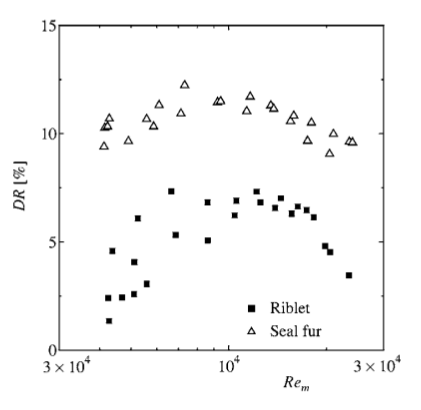
\includegraphics[width=0.5\linewidth]{chapter_1/seal}
\caption{$DR \% = \dfrac{ \Delta \tau}{\tau_{0}} \%$ Image from \citet{itoh2006turbulent}.}
\label{fig:seal}
\end{figure}


Compliant surfaces can in fact move accordingly to the surface pressure gradients along the boundary layer and so respond to the pressure fluctuation over the surface itself.
This mechanism is already know to be beneficial to delay the transition to turbulence and many authors have presented theoretical and experimental evidence on the effectiveness of this solution \cite{carpenter1990status}, \cite{bushnell1977effect}.

So we have seen that to reduce turbulent skin-friction drag riblets and natural surfaces uses various mechanism such as: sublayer vortices interaction, compliance and separation control.
Such solution have proven to be effective in some cases but they are related mostly in reducing the viscous component of the total drag.
In the next section we will introduce another class of solution that try to act instead on the pressure component.


\subsection{Permeable surfaces}

\subsection{Bluff bodies}

Permeable surface has been proposed to exploit even further the mechanism explained above using riblets.
There is some experimental evidence that in laminar cases the generation of some \textit{slip velocity}, at the interface between the permeable surface with the fluid , can decrease the friction drag \citet{beavers1967boundary}.
However in the turbulent case it seems that the instabilities developing at the interface can cause an increase in drag up to $40\%$ \citet{jimenez2001turbulent}, \citet{breugem2006influence}; this last mechanism will be further exploited in the section \ref{sec:stability}.
Is important to pinpoint that the permeable surface cited in the above references were all rigid.

The resistance pressure contribution is usually the most significant one in bluff bodies applications, and even in highly streamlined body it is around $10\%$ of the total drag.
Researchers have tried to find a way to modify the pressure distribution around a bluff body to reduce the associated resistance, and also dump the force oscillation on the body (drag and/or lift).

The pressure drag on a bluff body depends mostly on the difference between the low pressure on the rear part of the body, where there is usually a separated flow region, and the high pressure in the forward part.
This idea is sketched in figure \ref{fig:pressure_dist} where two different pressure distribution are shown; the black one represent the classical solid body, and the green one is the one with a porous layer at the back of the body.

\begin{figure}[h]
	\centering
	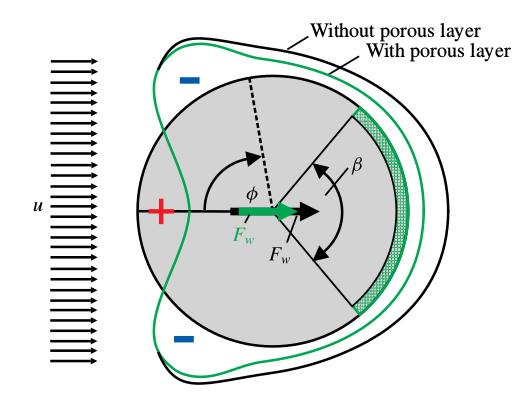
\includegraphics[width=0.4\linewidth]{chapter_1/pressure_dist}
	\caption{Diagram showing an example of pressure distribution around a cylinder for a viscous flow. The black line is the angular distribution as a solid body, the green one is the modified pressure in presence of a porous layer at the rear part. Image from \citet{klausmann2017drag}}
	\label{fig:pressure_dist}
\end{figure}

The favorable increase in the back pressure is due to the low speed laminar flow in the porous media that is ejected in the back region where the separation take place.
Even in very high speed turbulent flow the fluid inside permeable surface exhibit a very high energy loss due to the strong dissipation that the medium provide, resulting so in a low speed flow ejected downstream of the body.

The instability around a cylinder is due to the shear layer that forms in the top part of the body when the flow start to decelerate.
This shear layer exhibit a Kelvin–Helmeholtz type instability that develop in the classical Von-Karman wake.
The permeable interface, producing a slip velocity, can modify the boundary layer that develops above it and with that produce less shear and vorticity.

This two hypothetical mechanisms has been tested numerically numerically by multiple authors: \citet{bruneau2004passive}, \citet{bruneau2008numerical}, \citet{bhattacharyya2011reduction}, \citet{naito2012numerical}, \citet{mimeau2017passive}.
In their work they have add a porous layer to some classical two dimensional bluff bodies (cylinder, square cylinder, Ahmed body section, 3D hemisphere)and performed laminar and turbulent simulation for the flow around such bodies.

These works show some very strong result on multiple quantities, like: decrease of entstrophy, lower root mean square of the lift signal, drag reduction, regularization of the wake and lower pressure gradients; even if the porous medium is always rigid in their case.
An example is shown in figure \ref{fig:porous_cylinder} where the flow field downstream to a square cylinder is computed in a turbulent case; the picture show how the porous layer strongly regularize the wake.

\begin{figure}[h]
	\centering
	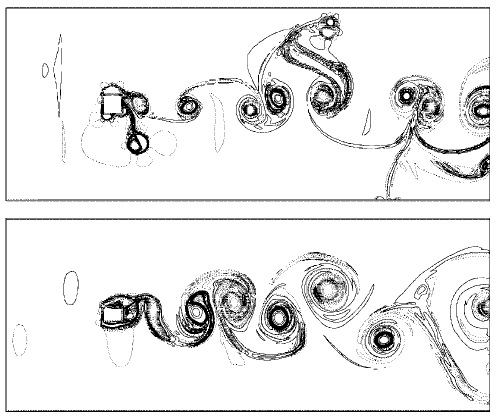
\includegraphics[width=0.7\linewidth]{chapter_1/cylinder_porous}
	\caption{Square cylinder vorticity countour for $Re=30000$. Top: solid case. Bottom: porous case with layer extension $h=10\% D$.}
	\label{fig:porous_cylinder}
\end{figure}


It seems from the previous works that the porous medium parameters, like the permeability (resistance) or its vertical extension, have important effects on the results.
They seems to agree (at least qualitatively) that increasing too the porous medium extension over a certain limit is not beneficial, and they also show that the resistance of the medium in order to be effective should not be excessive (medium to high porosity are the best).

In all these work we observe a reduced pressure drop between the front and the rear of the body, a reduced drag, delays in the vortex shedding in the laminar case and regularization on both the frequency and the amplitude of shedded vorticies oscillations.

These early work show very optimistic numbers but they should be taken with some care; only few cases are three-dimensional, and they all use a modeling approach for the porous medium based on a simplified version of the VANS (volume average Navier-Stokes equations, see section \ref{sec:vans}) without performing any validation of the method, and sometimes they use the equations outside their field of validity (there is some discussion in the scientific community in using such methods for highly turbulent flows).

The lack of validation reflect the fact that reliable experiment of such porous coatings are almost non existent in literature.
They also do not agree on the methods used to compute the forces \citet{caltagirone1994interaction}?? SHOW HERE THE GOOD METHOD ? MAYBE IN THE VANS SECTION...


\citet{favier2009passive} use a different numerical method that includes the dynamic of a moving porous medium made of fibers at the back of a cylinder.
Their results in a laminar flow case agree with the results on the stabilization of the wake and show some more realistic values of drag reduction, about $15\%$.
The difficulties in this model is in the medium dynamic, since it introduce many mechanical parameters that are not easy to identify for natural surfaces.

A similar model to the previous one has been used by \citet{venkataraman2012numerical}; the authors applied a movable porous coating in the top part of naca airfoil.
In this case the synchronization between the oscillations of the structures and the natural frequency of the fluid is responsible for the pressure distribution modification.
They have shown the robustness of this solution in a wide range of angle of attack, in the best case they have found some lift enchantment and regularization and a drag reduction has been measured to be on the order of $10\%$.

Later on \citet{rosti2017pelskin} works on a similar configuration with only one movable flap on the low pressure side of airfoil; the results both numerical and experimental qualitatively agree (on the flow mechanism) with the results in the complete porous case.


WHEN IT WILL BE PUBLISHED SHOW SOME RESULTS ON THE 3D SPHERE USING HOMOGENIZATION \citet{zampogna2017new}

The are very few experiment in literature on this porous coatings, but they all seems to show less promising numbers when  dealing with drag reduction.

For example \citet{heenan1998passive} perform an experiment in which he take a backward facing step with a porous insert in the re-circulation region.
His measurement show a $13\%$ decrease of the peak of pressure at the wall and a relocation of the detachment point further downstream.
Also depending on the length of the porous insert a maximum of $9\%$ of drag reduction was also observed.
The effect of adding a porous surface in this case was to limit the pressure fluctuations that causes the re-circulation bubble unsteadiness.

Later \citet{klausmann2017drag} study a 3D cylinder with a porous insert in the back; the authors use a wind tunnel testing with pressure measurements around the body and particle image velocimetry (PIV) flow capture.
Their results confirms that the porous layer on the leeward side increase of pressure in that zone, causing the reduction of drag.
The drag reduction measured to be around $10\%$ over various Reynolds number in the fully developped turbulence range, but it can be more sensible to the geometrical parameters of the medium as the position and its size.
At our knowledge this is the first example of actual measurements of flow quantities using PIV, that can later be used to perform some validation on different numerical models.

Some other experimental data can be found in the case of flow over aquatic canopies \citet{zhang2011exchange}, \citet{segalini2011experimental}, \citet{hamed2017impact}, even though the published data is limited and the problem in this case has also a free surface that increase the difficulty of the problem and limits the possible use as validation.

From this section the main physical mechanism that tied to permeable surfaces has been introduced but the different approaches in literature seems to be discordant in the predicted values of some fundamental items such as the forces.
Is it clear that the scientific community need much more experimental data in order to develop new and improved numerical and theoretical models for such permeable coatings.

\subsection{Canopy flow}

Another important class of flow over poroelastic carpets are the \textit{canopy flow} as known in literature; they are flow over flexible slender structure as threes or aquatic vegetations.
The importance of winds over plants is very important in a large variety of fields, like: the transport of substances as $CO_2$ and nutrients or preventing agricultural damage (windthrow of crop fields); also the above examples show some dynamic similarities even with urban canopies \citet{ghisalberti2009obstructed}.

It is known that the turbulent boundary layer profile over a canopy differ substantially from the rough wall one, figure \ref{fig:spectra}.
The vegetation resistance (drag) cause the creation of an inflection point in the mean velocity profile that lead to a mixing layer type of instability near the vegetation top.
In the work of \citet{finnigan2000turbulence} the author focused on the turbulent feature of the flow field in presence of vegetation.
He show that the vegetation can heavily modify the turbulence spectra as a results of the interface instabilities and the coherent structures above it.
As the two bottom pictures in figure \ref{fig:spectra} show, the spectrum in the case of canopy flow present a larger peak in the frequency of the mixing layer instability, a steeper slope in the energy cascade part due to the larger dissipation inside the permeable layer and possible high frequency peaks associated to the swinging of the pants that can emit or absorb small scales vorticies.
 
\begin{figure}[h]
	\centering
	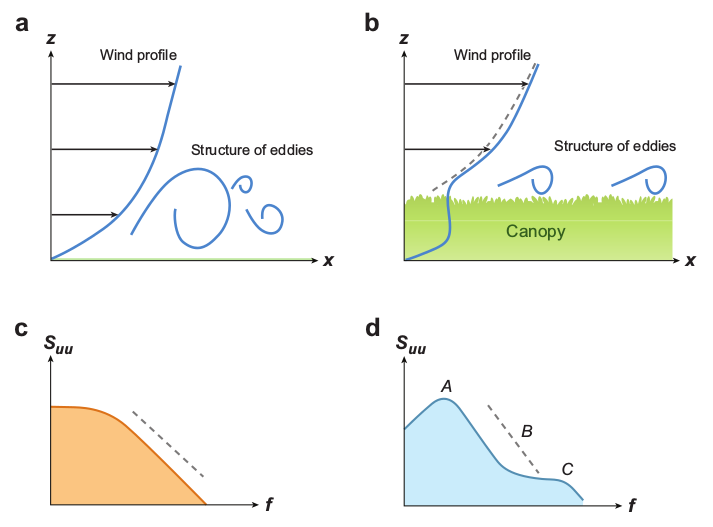
\includegraphics[width=0.7\linewidth]{chapter_1/spectra}
	\caption{bla bla \citet{de2008effects}}
		\label{fig:spectra}
	\end{figure}

So is it clear that the dynamic of the permeable substrate made by vegetation is extremely important and should always take into account to fully generalize the physics in such problems involving moving canopies.
As shown in \citet{nepf2012flow} especially for aquatic plants the movements of the plants can be important and so the interface can be largely modified.

In order to discriminate the different behavior of the fibrous structure we need to introduce some important non dimensional parameters used in fluid structure interaction problems:
$$ m^* = \rho_{\beta} / \rho_{\sigma}, \quad C_Y= \rho_{\beta} U^2 s^3 / E, \quad s = L/\ell $$
The first one is the mass ratio, the second is called Cauchy number and the last one is the slenderness of the structure.
The mass ratio $m*$ is a measure of the added mass effects caused by the solid inertia, but this effects are usually negligible in case of fibrous permeable media.
The Cauchy number $C_Y$ define the static deformation of a solid caused by the fluid flow ($E$ is the modulus of elasticity of the solid material), at Cauchy numbers over the unity important deformation are expected.
This number is extremely important since it control a phenomena called \textit{reconfiguration} that leads to drag reduction \citet{gosselin2011drag}, \citet{alvarado2017nature}.
The reconfiguration is the capability of the structure to adopt a new shape when forced by a flow, it can become more streamlined and/or reduce its exposed frontal area with the aim to reduce the total drag.
When dealing with this phenomena we should take together the frontal area $A$ and the drag coefficient $C_D$ to avoid misinterpretation of the drag reduction; in figure \ref{fig:cycd} this ratio has been represented for different natural structures against the Cauchy number and is it clear that for a $C_Y>1$ we have a drastic drag reduction.

\begin{figure}[h]
	\centering
	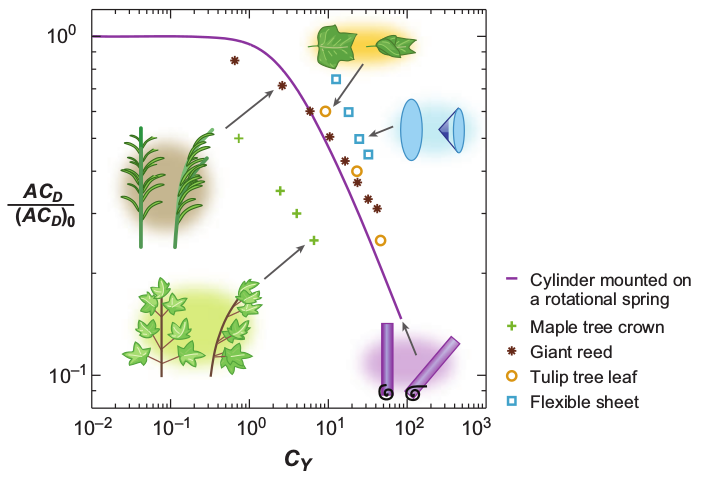
\includegraphics[width=0.7\linewidth]{chapter_1/cy_cd}
	\caption{The effect of the Cauchy number $C_Y$ on the drag reduction are presented in the figure. The drag reduction has been represented has the ration between the frontal area $A$ and the drag coefficient $C_D$ at static condition (subscript $0$) and the dynamic condition. Image from \citet{de2008effects}}
	\label{fig:cycd}
\end{figure}

The overall reconfiguration of the permeable medium can lead to pressure recovery and a wake regularization applied to a bluff body, as the experiments by \citet{gosselin2011drag} show.

Another important non dimensional number is the \textit{reduced velocity} and it can be derived form the previous ones as:
$$ U_R = \sqrt{C_Y s / m^*},$$
this number is used dealing with vortex induced vibration of slender structure, if it is in the order of unity it means that some dynamical coupling between is expected such as resonance or lock-in.

Canopies can help to prevent separation in presence of adverse pressure gradients, \citet{belcher2012wind} show an analysis of the flow over an hill covered with canopies using either numerical and experimental data; the authors show how the permeable layer can present a recirculation region inside the canopy in the decreasing slope side of the hill, so moving the separation from the flow over the hill to the internal structure of the canopy.
In this sense when we look at the "global" hill (ground and canopy layer) the reversed flow typical of this geometry is not present.

Is important to pinpoint that the above results are restricted to fibrous or slender structure, and they cannot be extrapolated in general for all different porous structure ans shapes, even though similar mechanism are expected.

In the case of canopy flow is very difficult to compare results because most of the authors use very different models in a lot of regimes of velocities and using flexible structure with very different shapes.
Even if much more experiments are available \citet{segalini2011experimental}, \citet{segalini2013scaling}, \citet{maza2013coupled}, \citet{barsu2016drag}, \citet{alvarado2017nature}, there is no quantitatively mathematical model established for the fluid and structure equations and most of them rely on empirical correlations that fit the data of each different case.


\section{Models for flows through porous surfaces}

In this section we want to state clearly what is the problem that we are trying to solve and which characteristic are the difficult one.
In order to be as clear as possible we have taken the simplest example to define the problem; the flow over a wall that include multiple flexible filaments. 
This is probably the simplest geometrical configuration to think about but it still has all the characteristic and difficulties of more interesting configuration, such as a bluff body with a poroelastic layer.

\begin{figure}[h]
	\centering
	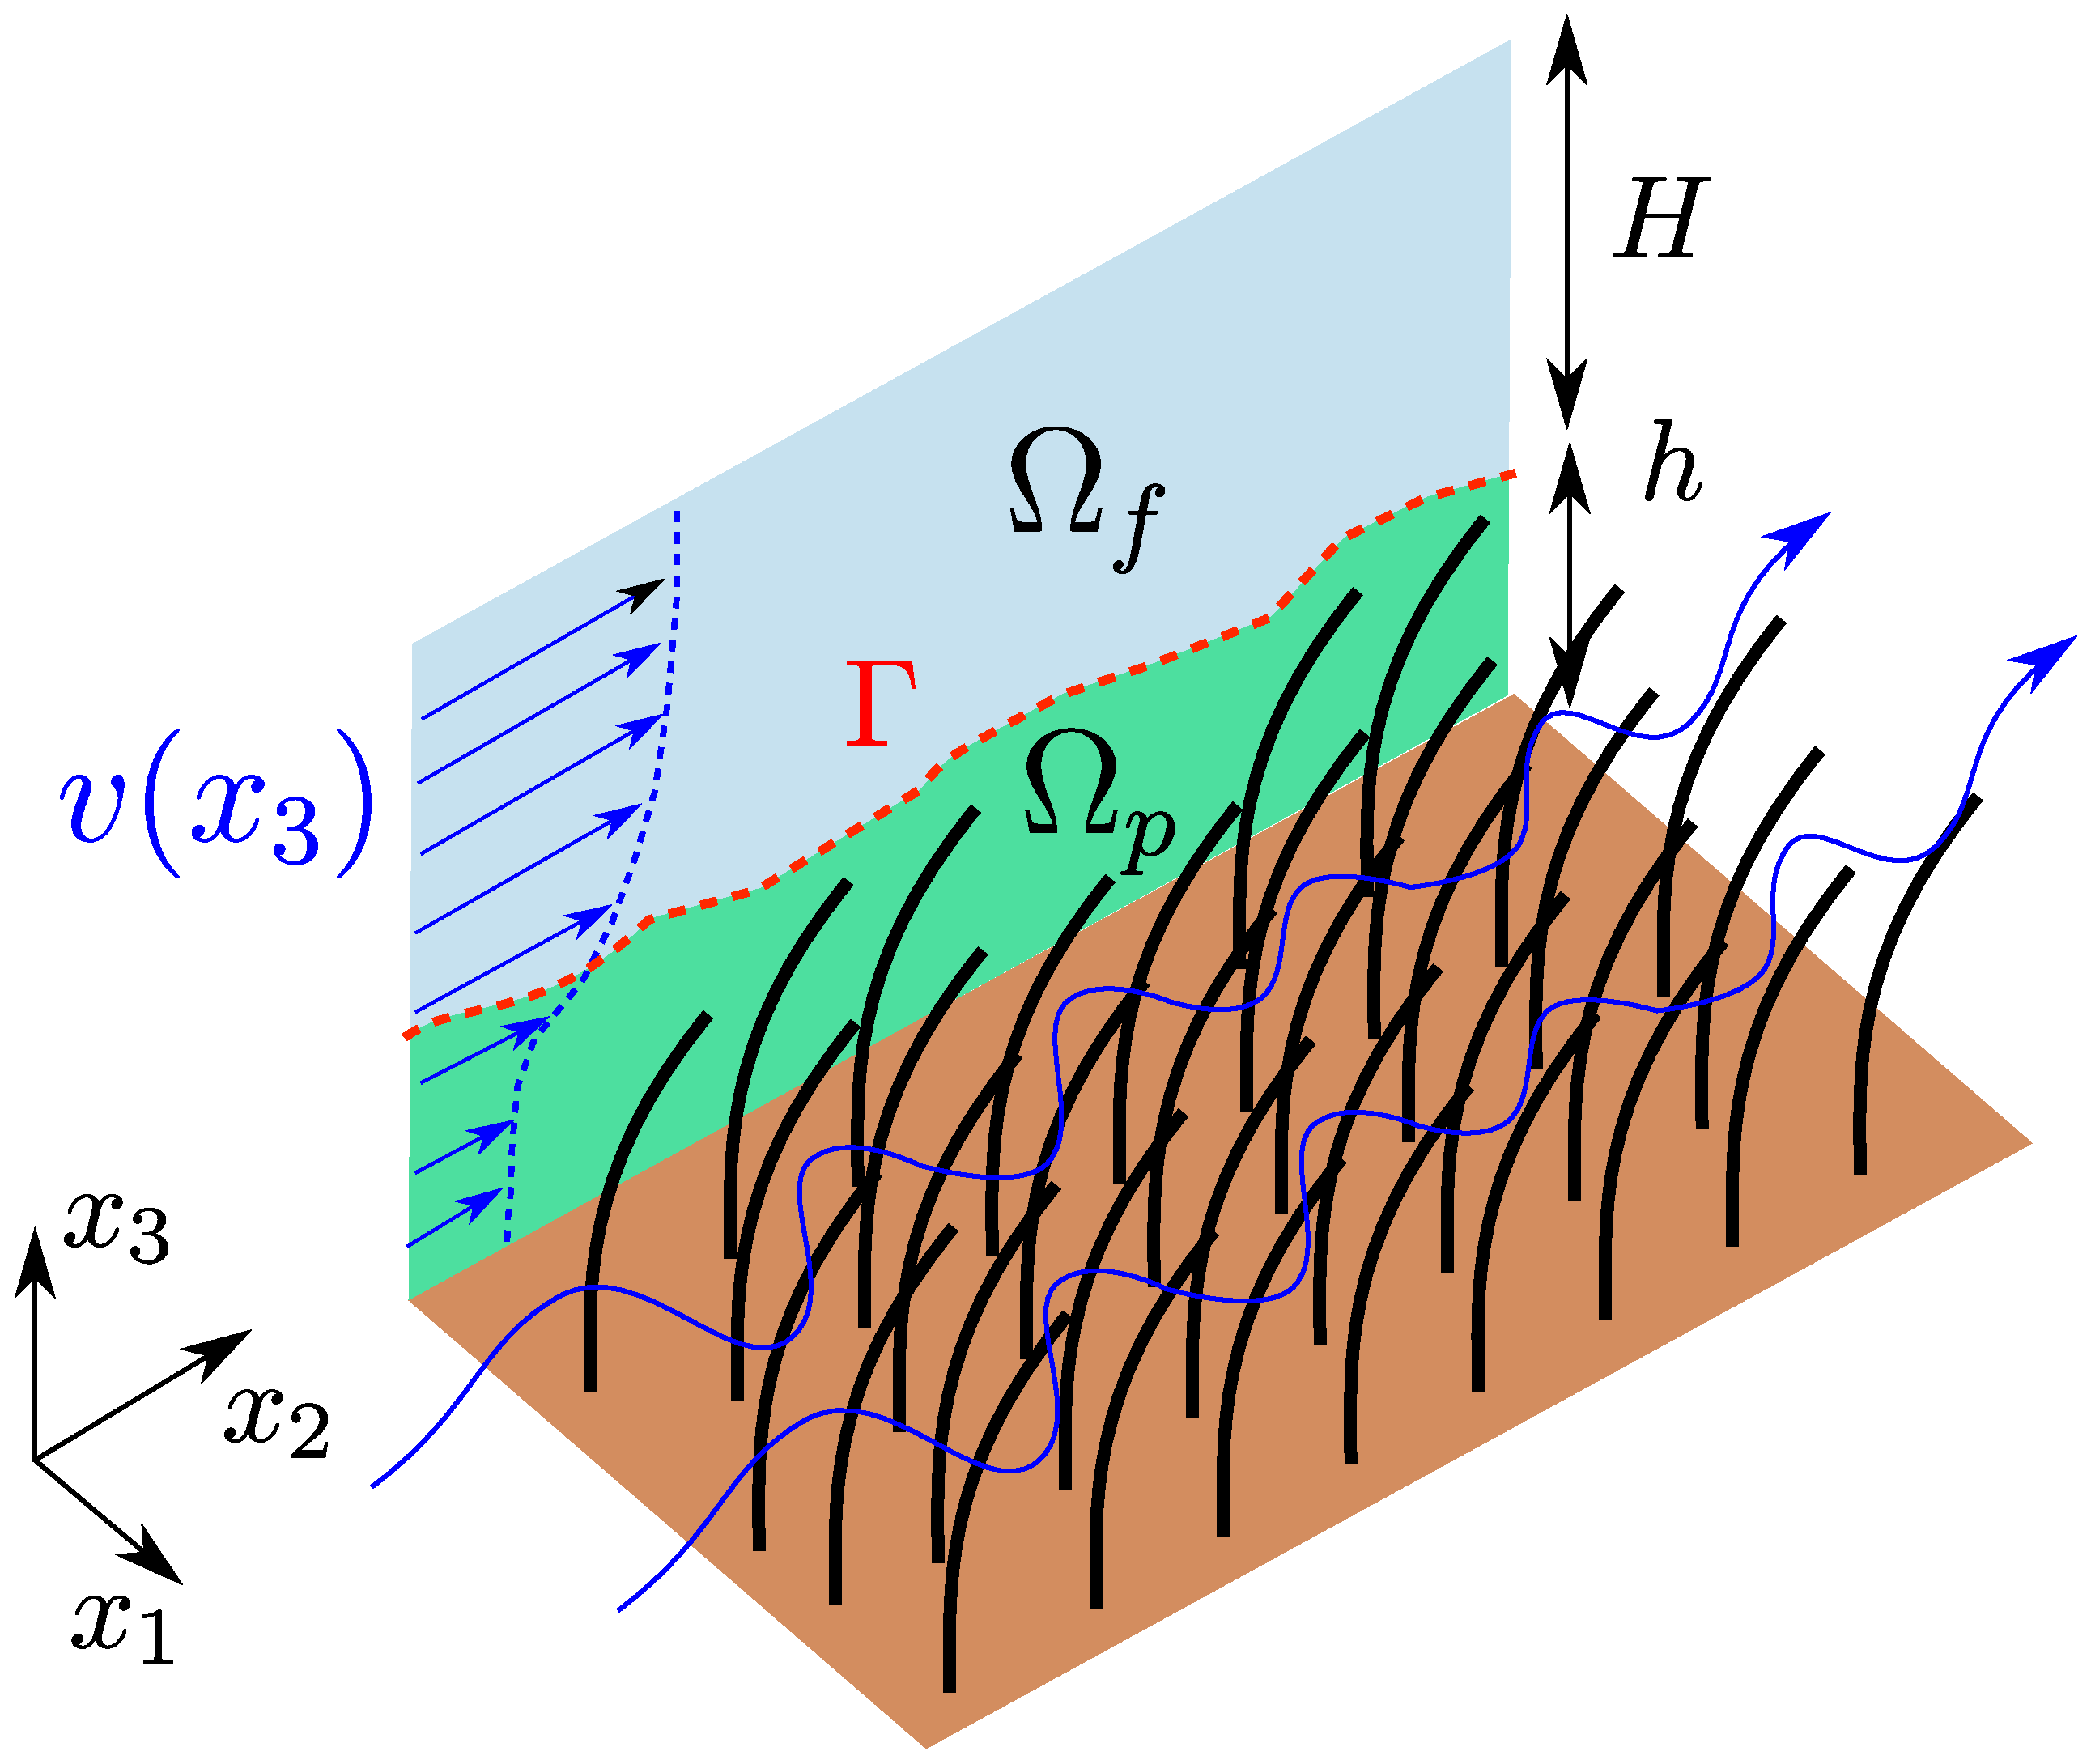
\includegraphics[width=0.7\linewidth]{chapter_1/problem_schema}
	\caption{Sketch of the fully developed flow over a poroelastic surface made of multiple filaments.}
	\label{fig:schema_problem}
\end{figure}

The figure \ref{fig:schema_problem} show a graphical schema of such flow; the fluid main direction is aligned with the $x_2$ axis and the projection of the streamwise component is shown in the plane $x_2 - x_3$.
Such flow can bend the filaments and, of course, pass through their ensemble.
The hypothetical surface that envelop all the filaments ends ($\Gamma$), defines the limit between the flow without obstacle ($\Omega_{NS}$) and the one inside the poroelastic medium ($\Omega_{P}$), their projection are shown in the  $x_2 - x_3$ plane.

In order to computationally solve this problem there are some key points:
\begin{itemize}
	\item Length scales: the flow is very rich of multiple scales vorticies. The flow can have KH instabilities on the interface (that has the size of $h$) but they can even penetrate inside the medium and brake up to very small scales. In order to resolve this complex dynamic one should have a very fine mesh (very computational expensive) or came up with a model (like in turbulence).
	Also the turbulence dynamic can be a problematic; the hypothesis that turbulence can exist in porous media is still at debate in the community.
	Deal with such small scale dynamic and find a model for at least the interface part (in which the KH vorticies forms and brake up) is not an easy task.
	
	\item Compliance (Fluid structure interaction): if the filaments are flexible they bent and swing due to the fluid force that act on them.
	We have to take into account a mechanical solid model for the filaments such as the Bernoulli beam, and compute the energy that the swing of the filaments will re-inject inside the fluid flow.
	This two-way coupling could be also really computational expensive in presence of a large number of filament structures, and also if the the filaments are really flexible one should in principle take into account the possibility of contact and repulsion between the fibers.
	If the medium has a much more complicated shape (like the scales in the butterfly) one probably cannot use simplified models sor the solid dynamic and so use a general FEA discretization on the solid that is even more expensive.
	Another approach consist of consider a general model for the medium, for example treat it like a porous medium that can have elastic properties.
	Such models mimic the dynamic of the solid and in theory are more adapted to porous media that are fully connected, in principle they are very computational convenient but their mathematical description can e difficult and one should agree on the idea of losing information inside the medium.
	
	\item Anisotropy: the problem should be capable of treat permeable surfaces that have different response when stressed in different directions. For example the geometrical disposition and/or the mechanical properties of the medium can be non homogeneous, so the medium will be more permeable in one direction and so have a preferential flow path.
\end{itemize}

Examples of full resolved fluid-structural problem in which either the flow and the filaments structure has been resolved directly are very few in literature.
\citet{marjoribanks2017does} performs large eddy simulation over a bed with $300$ filaments; but he use a very simple drag model for the fibres mechanics and use a one way coupling between the solid and the fluid, so he resolve the fluid, pass the forces on the solid, compute the new solid position and directly go to the next time-step without re-iterating.
Even with a simple coupling and solid dynamics the flow show some insight in the fibers dynamic, but again the lack of validation makes the results questionable.

\citet{dupont2010modelling} previously made a similar model introducing a two way coupling for the fluid-structure interaction problem, this time they validate their code with video recording of a similar experiment and the frequency measurements of the KH instabilities at the interface agrees very well.
The authors so not give quantitative information of the computational configuration but mention a very important high performance computing center in the acknowledgment which made us suppose that the computational power involved were substantial.

Show other examples that solve directly the full coupled problem are in \citet{pinelli2017pelskin} \citet{favier2017pelskin}, \citet{revell2017pelskin} but in this case the number of filaments is small and so they can be though more as singular filaments that a really poroelastic medium.

There is of course another way to treat the problem state ìt above that does not use \textit{brute force}.

Due to the computationally expensiveness on solving the problem directly the scientific community has came out in time with different approaches that treat the porous domain with a generalized model that do not resolve the fine scale inside and between the filaments but instead express them as a function of the length scales present in the fluid domain $\Omega_{NS}$.

The key point in such methods are:
\begin{itemize}
	\item They divide the overall domain in two different parts: the fluid domain $\Omega_{NS}$ and the porous domain $\Omega_{P}$
	\item Two different fluid models are solved in the two domains, in $\Omega_{NS}$ the Naver-Stokes equations for incompressible fluids are the classical choice, and in the porous part there are a number of different models that usually neglect the temporal derivative and the convective part in the latter equations but adds other source terms in order to take into account the presence of the solid inclusion that form the porous medium
	\item The two domains are coupled together with an interface boundary condition or a special equation treatments for this transition region
	\item A model for the dynamic of the solid porous part should also be chosen
\end{itemize}

Also the interface treatment and the solid model can be tied to the choice of the porous fluid model.
The source term introduced in $\Omega_{P}$ depends on the theory in which we develop our porous media model, in the next two section we will talk about the two main branches existing in literature.

\subsection{Isotropic drag models}
\label{sec:canopy_eq}

In the case of flow through vegetation (canopy flows) it is common to use a simpler isotropic drag model for parametrize the resistance of the canopy.
So the drag is usually function of the depth (the distance from the interface in the wall normal direction) and it is supposed to be isotropic; this hypothesis can be correct in case of dense vegetation when the flow cannot generate almost any wake inside the canopy, but it is certainly wrong in the wall normal direction since for a flow purely vertical the resistance of the medium should be smaller.
However since this models are mostly applied in channel problems where the mean flow is mostly streamwise the resistance in the vertical direction can be approximated in this manner, but in application where the transpiration of the interface is important (wake control of bluff body) the isotropic drag model is certainty not convenient.

The drag resistance is included in the incompressible Navier-Stokes equations as a sink of momentum as in equation \ref{eq:mom_cd}.

\begin{equation}
\derp{\vb}{t} + \vb \cdot \nabla \vb = -\frac{1}{\rho_{\beta}} \nabla \pb + \nub \nabla^2 -C_D a |\vb| \vb, 
\label{eq:mom_cd}
\end{equation}

The sink term is quadratic in the velocity but there is some evidence that the reconfiguration phenomena can change this relationship taking into account the drag reduction \cite{gosselin2011drag}, \citet{alvarado2017nature}.

The sink term includes also the parameter $a$ that is the frontal area per unit volume of the vegetation and even if it has the dimension of a length this parameter is an expression of the porosity of the medium.

For our point of view this approach lack of strong mathematical formalism, from which one should be able to derive all the additional terms of the equations; as a consequence, this method heavily rely on empirical relations.
One other problem is that the isotropic hypothesis rule out the possibility to model the anisotropic nature of most of the surfaces in which we are interested (as equation \ref{eq:max_dr} suggest the difference in the permeability in different directions can be important for the drag reduction).

But in the field of vegetations a lot of authors have successfully used this approach in various domain, for example \citet{maza2013coupled}, \citet{maza2015tsunami} use it to study wave attenuation, \citet{ghisalberti2004limited}, \citet{battiato2014single} develop a simple model for the 2D mean flow over a canopy.


\subsection{Homogenization models}

The above section introduce the idea to look at the problem as it was composed by two different domains; here in this section we want to introduce the most used approach to derive the equations that are valid in the porous domain in an \textit{averaged} sense.
The fundamental idea is to construct a micro-scale model, either for the fluid as for the solid, and then derive the macro-scale equations using some averaging operator over the micro-scale.

The two most known homogenization methods are the \textit{Volume Averaging} method \citet{whitaker2013method}, and the \textit{Multiple Scales} method \citet{mei2010homogenization}; they can be more broadly classified as perturbations methods. 
The key differences and the main results retrieved within this approaches will be presented in the following.


\subsubsection{Volume Averaging}
\label{sec:vans}

The method of Volume Averaging has been developed to threat transport equation in porous media applications; in this case the presence of two different length scales is obvious as in figure \ref{fig:porsystem}.
	
	\begin{figure}[h]
		\centering
		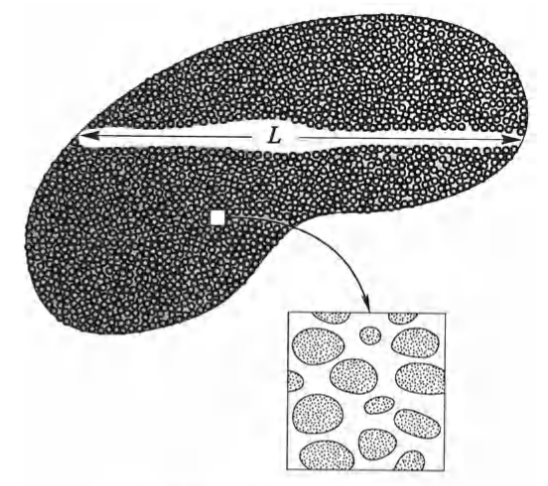
\includegraphics[width=0.7\linewidth]{chapter_1/por_system}
		\caption{dfdfsfd}
		\label{fig:porsystem}
	\end{figure}

The core idea of the methods is that we can firstly define an average operator as \eqref{eq:avg_intrinsic_intro}, in this case the variable $\psi$ can be any vector or scalar variable in the sistem of equations that we want to homogenize, for Navier-Stokes it will be the velocity and the pressure.

\begin{equation}
\meani{\psi} = \dfrac{1}{\volb} \int_{V} \psi \, d \, V,
\label{eq:avg_intrinsic_intro}
\end{equation}

The average operator has the purpose to "scale up" the equation, in fact the second crucial step of the method is to decompose the variables as proposed by \citet{gray1975derivation}:

\begin{equation}
\psi =   \underbrace{ \meani{\psi} }_\text{O($L$)}  +  \underbrace{\tilde{\psi} }_\text{O($\ell$)},
\label{eq:vans_decomp}
\end{equation}

The \eqref{eq:vans_decomp} show how each variable can be decomposed in an averaged part that contains only spatial variation at the macro-scale $L$ and a \textit{fluctuation} part that contains only the micro-scale $\ell$ spatial variations.

The decomposition can be injected in the transport equations that we want to homogenize, and new transport equations that includes only variables of order O($L$) can be retrieved.
Since this is the method chosen to solve our problem, all the technical details will be detailed explained in the chapter \ref{ch:vans}.

The most famous application of the method is the Stokes flow inside a rigid porous medium as the one in figure \ref{fig:porsystem}, the $\beta$ subscript indicate the liquid phase:
\begin{equation}
0 = -\dfrac{1}{\rho_{\beta}} \nabla \pb +\nub \nabla^2 \vb
\label{eq:stokes}
\end{equation} 

Here is important to note that the equation \eqref{eq:stokes} is valid only in the liquid phase and to solve it we have to consider all the solid phase as rigid boundaries, with the difficulties that came to define the complex structure of the solid inclusion.
Applying the Averaging Method we can derive an homogeneous version of the \eqref{eq:stokes} that is valid in the all the porous domain that include the two different phases, the solid and the liquid one; the famous Darcy equation \eqref{eq:darcyeq} \citet{whitaker1986flow}.

\begin{equation}
\vbmi = -\dfrac{\mathbf{K} \varepsilon}{\mub} \nabla \pbmi
\label{eq:darcyeq}
\end{equation} 

In the Darcy equation is possible to recognize two additional quantities that arise from the averaging procedure, the fist one is a scalar called porosity $\varepsilon$ and represent the ratio of the liquid phase present in a reference volume of the medium.
The second one is the tensor $\mathbf{K}$ called permeability, it express the resistance of the porous medium that affect the flow in its travel.
The term $\mathbf{K}$ play the same role as $C_D a$ in the isotropic drag model; but the main difference is that the permeability tensor can be computed directly from the geometry of the medium (see chapter \ref{ch:vans}) so it does not rely on empirical relations.
Also the tensorial nature of this terms permits us to model porous inclusion that are anisotropic in nature.

Applications of the theory include: fluid inertial terms \citet{whitaker1996forchheimer}, porous media with small deformations \cite{whitaker1986flow2}, and high deformations \citet{hussong2011continuum}, turbulence \citet{soulaine2014}, \citet{breugem2006influence}, interface between a permeable medium and a free flow \citet{beavers1967boundary}, multiphase systems \citet{whitaker1973transport}, heat transfer \citet{carbonell1984heat}.

Here we do not want to go into details of the derivation of equation for our specific problem but we want just to be clear about the differences of this method to the isotropic drag model of the previous section.
One of the greatest differences is the robustness that came from a mathematical formalism instead of an approach rely heavily on experimental closure terms.

\subsubsection{Multiple Scales}

The multiple scale method is similar to the previous one; and it has also been applied to similar problems in the context of porous media applications.

In this method we start with the assumption of scale separation between the two length scales, $\ell$ micro-scale and $L$ macro-scale; the scale separation factor can be defined as $\epsilon = \ell/L \ll 1$.
Using the same examples as before we want to show the how to compute the homogenized version of the Stokes equation for fluid flow through a porous media.
We introduce the micro-scale and the macro-scale coordinates of the problem defined respectively as:
$$
 X_i = \dfrac{\tilde{x_i}}{L}, \quad   x_i = \dfrac{\tilde{x_i}}{\ell},
$$
where $x_i$ are the original coordinate of the problem.
Using the above separation factor is possible to expand the variables of the problem (pressure and velocity) into orders (like a Taylor expansion) indicated with the number as superscript:
$$
\psi(X_i, x_i) = \psi^{(0)}(X_i, x_i)  +\epsilon \psi^{(1)}(X_i, x_i) +\epsilon^2 \psi^{(2)}(X_i, x_i) +O(\epsilon^3),
$$
injecting this decompositions inside the equation \eqref{eq:stokes} is it possible to derive a set of system of equations for each order of the expansion.
It can be shown that analyzing each equation in the set we can retrieve the homogenized equation:

\begin{equation}
{v_i}^{(0)} = -K_{ij} \dfrac{\partial p^{(0)}}{\partial X_i}
\label{eq:darcy_ms}
\end{equation} 

In which either the pressure and the velocity fields appear only at the order zero, and the equation depends only on the macro-scale length.

We find the same permeability tensor $\mathbf{K}$ as before, and its definition is the same.
So it is clear that for this example problem we find as results the same set of homogenized equation; it only change the starting hypotheses of the method and the mathematical development to compute them.

A full analysis of the dualism of the two approaches can be found in the work by \cite{davit2013homogenization}.

The multiple scale also has been used in \citet{zampogna2016fluid}, \citet{ugis}, ... FINISH THE APPLICATIONS IN THE LITERATURE


Is also worth mention another homogenization based method called mixture theory, based on similar approach is it possible to retrieve the same equation as the previous two methods \citet{rajagopal2007hierarchy}.




\section{Stability of flow over permeable surfaces (monami/honami and Kelvin-Helmholtz)}
\label{sec:stability}

\citet{finnigan2000turbulence} \citet{jimenez2001turbulent}

\subsection{Stability theory generalities}

In order to study some of the characteristic of the instabilities that develops at the interface of the permeable surfaces we have used the linear stability analysis; this methodology is part of stability theory that covers the modelling of the stability and transition of fluids flows.
We hare interested in this approach because it's a simple mode to compute the main frequency of the unstable mods of the canopy flow, the monami, and it is also possible to see if the porous flow can change the stability property of the flow introducing more unstable modes that doesn't exist in the flow without the canopy bed. 
 
We have limits our study in the local modal stability theory, basically given an operator that describe the evolution of small perturbation, is possible to study the spatial or temporal evolution of the individual eigenmodes of that operator.
The procedure of the linear stability relies on the decomposition of the flow quantities $\mathbf{q}$ into a steady state part $\overline{\mathbf{q}}$ called base flow, and an unsteady part $\widetilde{\mathbf{q}}$:

$$ \mathbf{q} (\mathbf{x},t)= \overline{\mathbf{q}} (\mathbf{x}) + \epsilon \widetilde{\mathbf{q}} (\mathbf{x},t) $$

Than the unsteady part is chosen to have this general wave form:
$$  \widetilde{\mathbf{q}} =  \widehat{\mathbf{q}} e^{i\Theta} $$

where the $\widehat{\mathbf{q}}$ it's the amplitude and the $\Theta$ is the phase of the perturbation.
The assumption made in base flow determine the choice of the amplitude and the phase function, so it change the stability theories, in the table below the main theories are classified:

\begin{figure}[h]
	\centering
	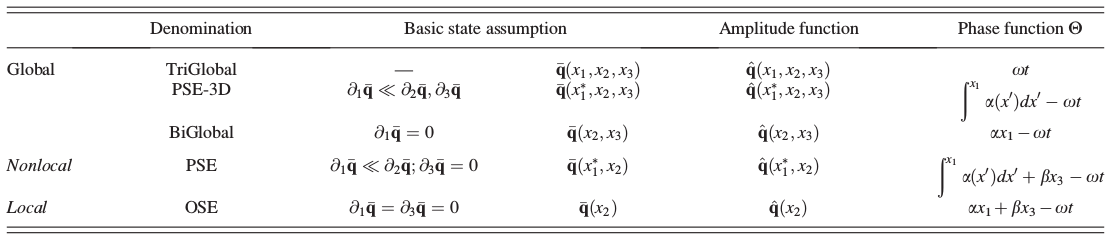
\includegraphics[width=1\linewidth]{chapter_1/table}
	\caption{Classification of modal linear stability theories}
	\label{fig:table}
\end{figure}

We have mainly use the simple linear local theory for our computation, that involves only one free direction and the other two has been taken as periodic:
$$  \widetilde{\mathbf{q}}(\mathbf{x},t) =  \widehat{\mathbf{q}}(x_2) e^{i(\alpha x_1 + \beta x_3 - \omega t)}  $$ 
where:
\begin{itemize}
	\item $\alpha$ is the streamwise wave number
	\item $\beta$ is the spanwise wave number
	\item $\omega$ is the wave phase
\end{itemize}

In our case we chose to have the wavenumbers real and the wave phase imaginary in order to perform a temporal stability study, introducing this decomposition inside the Navier-Stokes equations and linearise the problem is it possible to transform it into a generalized eigenvalue problem:
$$ A \widehat{\mathbf{q}}=  \omega \widehat{\mathbf{q}}B $$   

The above explanation is quite condensed but a lot of good literature has been developed in these years, \cite{juniper2014modal}, \cite{criminale2003theory}, \cite{schmid2012stability}, in which there is also a good review of the computational algorithms needed to solve the problem.

\subsubsection{Porous Medium applications: monami/honami}

\citet{inoue1955studies} first to talk about monami /honami

CONTROLLA INTRO CAPITOLO 3 MAGARI C?é GIA QUALCOSA
\citet{pluvinage2014instabilities}
\citet{py2006frequency}
\citet{singh2016linear}

figure from Finnigan
figure from Nepf


\begin{figure}[h]
	\centering
	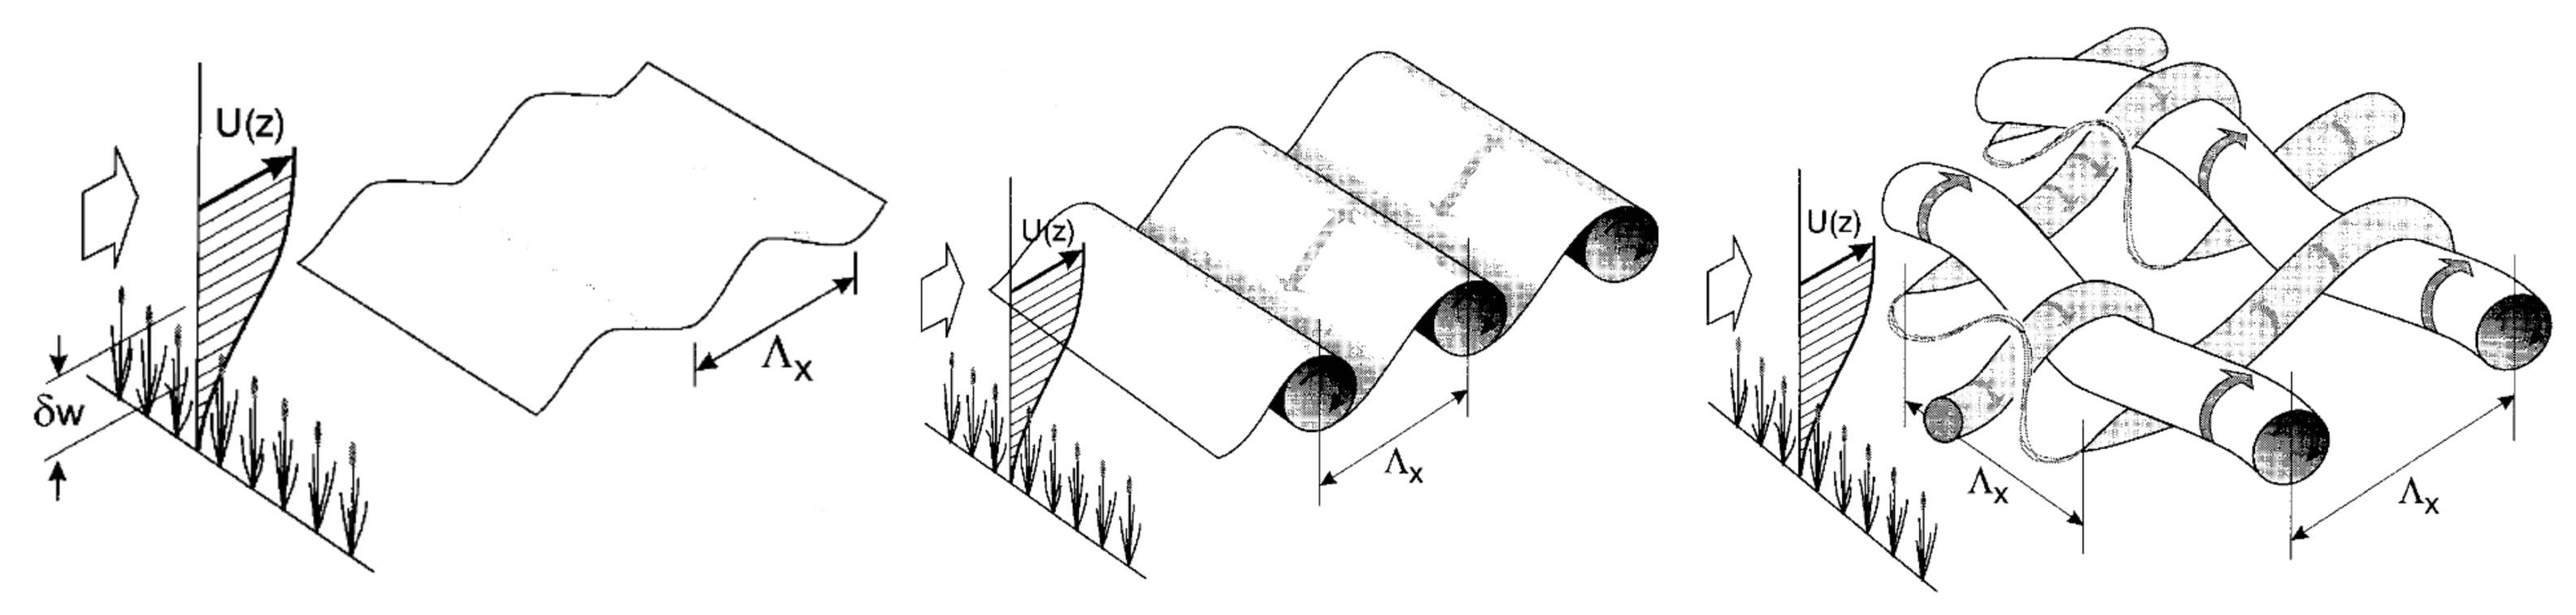
\includegraphics[width=1\linewidth]{chapter_1/finn}
	\caption{Monami, honami .... Image from \citet{finnigan2000turbulence}}
	\label{fig:monai_evol}
\end{figure}


The above framework for the stability problem of fluids has already been applied in some porous media flow configurations. 

\citet{avramenko2005investigation} have studied the stability of a Poiseuille flow with all the channel taken as a porous medium, using the Darcy-Brinkman-Forchheimer equation, they have found that the increasing of porosity stabilize the fluid flow and also the Forchheimer correction do the same. 

The two works \citet{tilton2006destabilizing}, \citet{tilton2008linear}, expose a very good explanation of all the physics and all the parameters involved in the stability of these type of flow, in particular they analyse the Poiseuille flow in the case of either the presence of a porous layer on the bottom of the channel or the presence of this porous layer in the top and in the bottom as shown in the figure below:

\begin{figure}[h]
	\centering
	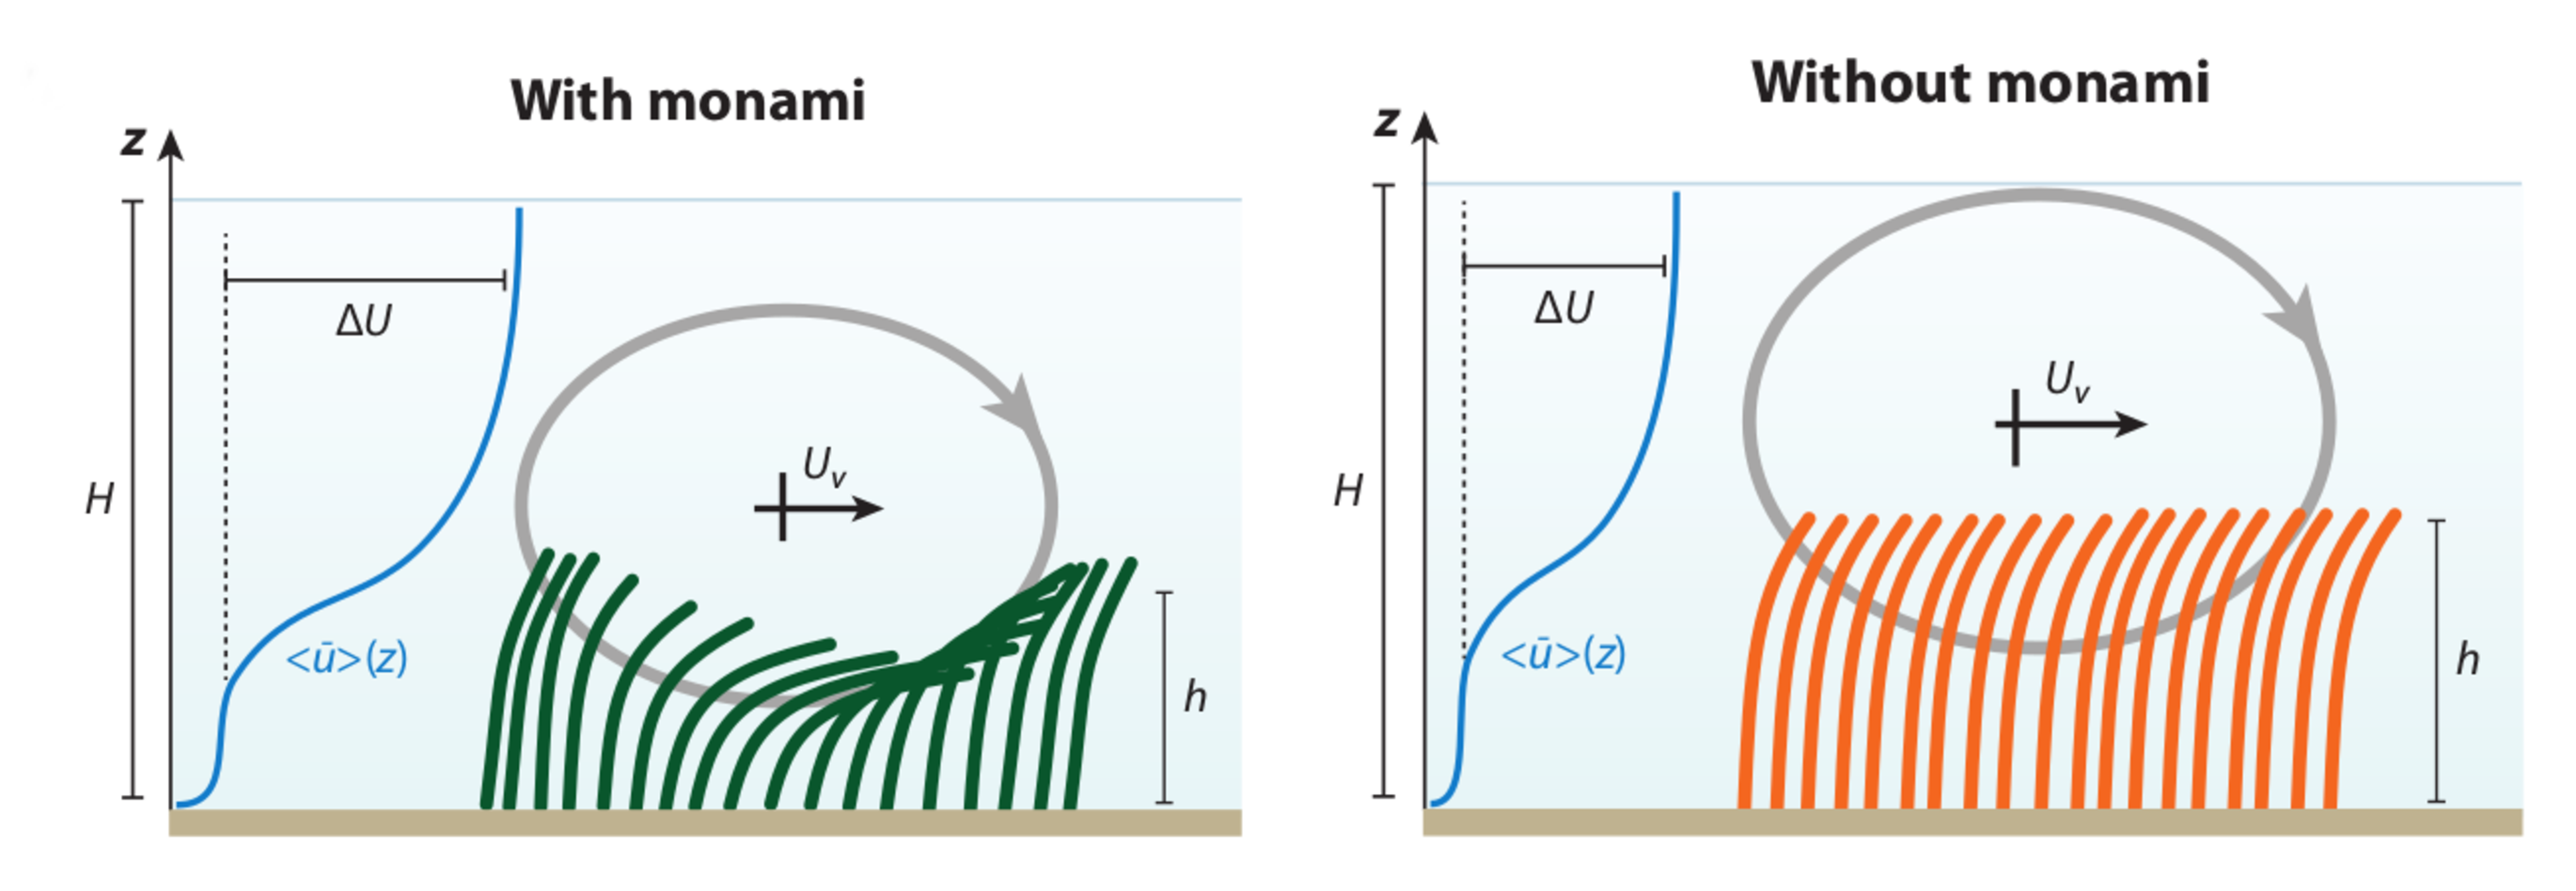
\includegraphics[width=1\linewidth]{chapter_1/monami}
	\caption{Monami, honami .... Image from \citet{nepf2012flow}}
	\label{fig:monami}
\end{figure}

They have used The Darcy-Brinkmann equation and the Ochoa-Tapia interface condition to derive either the base flow and also the stability equations, but in the latter they drop the Brinkman term.
They have studied a lot of aspects of the linear stability problem:
\begin{itemize}
	\item difference between the presence of one or two porous layers
	\item height of the porous medium layer compared to the channel one
	\item porosity 
	\item coefficient of the shear stress jump in the interface condition
	\item inertial effects in the proximity of the interface (Forchheimer correction)
	\item effects of the use of the Darcy only equation (this imply to have a discontinuity of the velocity profile at the interface)
\end{itemize}

It's shown that the porous layer trigs new unstable modes, reducing a lot the critical Reynolds number. 
The results are very detailed and seem to be in good agreement with some experimental data, also the results of \citet{chang2006instability} are qualitative comparable even if in the previous paper the authors express some criticism in the results of Chang because of some bad assumption.


Another application of the linear stability can be found in \citet{white2007shear} in which some experiment of a flexible canopy bed are compared with a linear stability analysis this time in the spatial framework; the results of the theory seems to be in agreement with the experiments.
